\chapter{NC Experiment 2}

\section{Design}
\paragraph{}The purpose of the second experiment was to compare the NC to a generic WDRC hearing aid, while controlling for as many other factors as possible that could contribute to a person's preference of hearing aid.  The hearing aids were equated in physical appearance, hardware (both used the GA3280 microprocessor platform), and any supplemental features, such as noise reduction and feedback cancellation.  The implementation of the noise reduction system on the NC and WDRC hearing aids was identical, but there were slight differences in the implementation of the feedback canceller, though they used the same resources on the microprocessor.

Figure 5.1 shows a week by week schematic of the study design.  The study was double-blind, such that both the experimenter and the participant were unaware of which set of hearing aids a participant wore at any given instant.  At the very beginning of the study, participants were issued a structured diary.  The structured diary was of a similar format to that used in \citeA{Moore2005}, and there were four forms in the diary to be filled out on particular dates.  These forms asked participants to rate the loudness and clarity of target speech and the loudness of background noise for six different situations (e.g. car, having a meal with 2-3 people, etc.), as well as to report how many hours per day they wore the hearing aids.  In addition to the structured part of the diary, there was also a freeform section, where participants were asked to take note of any unusual sounds, any instances of feedback, and whether any sounds were too loud or too quiet.

\begin{figure}[htp]
\begin{center}
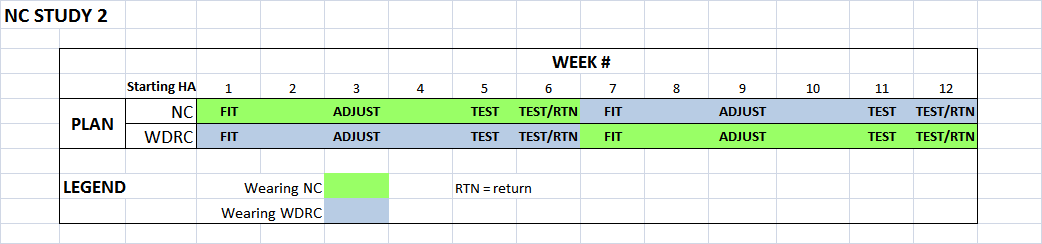
\includegraphics[width=\textwidth]{chap5-design.png}\\
\caption[NCStudy2 design]{NCStudy2 design.  Half of the participants were fit with WDRC hearing aids at the outset of the study, while the other half were fit with NCs.  Adjustments were given 2 weeks after the initial fit.  Halfway through the study, participants returned their current set of hearing aids in exchange for the other set of hearing aids, which were fit to their loss.  Two test sessions were conducted for each pair of hearing aids.}
\label{ch5-design}
\end{center}
\end{figure}

Roughly half of the participants (6) were randomly assigned to begin the study wearing the WDRC hearing aids, while the other half (5) were fit with NC hearing aids.  After a two week period of wearing the hearing aids (deemed the first adaptation period), the participants visited McMaster, and were given an adjustment to their hearing aids by a trained hearing instrument specialist (HIS).  After the adjustment, participants wore the hearing aids for another two weeks (the second adaptation period) before coming in for two, two hour test sessions, spaced one week apart.

Adjustments were guided by observations that participants had recorded in their diaries, as well as from verbal reports given by the participant at the time of the adjustment.  Following the second test session, participants who first wore NCs returned the set of NCs, and were lent out a set of WDRC hearing aids, while participants who first wore a set of WDRC hearing aids were given a set of NCs.

\section{Participants}

\subsection{Demographics and Prior Experience}
\paragraph{}A total of 11 participants qualified for the study (7 male, 4 female), with an average age of 70.5 (SD = 9.6).  None had prior experience wearing hearing aids, and all spoke English as their primary language.  The hearing aids used for the study were receiver-in-the-canal (RIC) style.

\subsection{Audiograms}
\paragraph{}Prior to their inclusion in the study, participants visited McMaster University for a hearing test; air conduction thresholds for both ears and bone conduction thresholds for the worse ear were measured.  A trained student performed the measurements, following the British Society of Audiology recommended procedure for pure-tone audiometry \cite{BSA2004} as closely as possible.  Tympanometry was also performed, to screen for normal middle ear function, as indicated by a Type A tympanogram according to the Jerger classification.

To qualify for the study, participants were required to have symmetrical sensorineural hearing loss, which was defined as: 1) no difference greater than 10 dB HL between ears on the calculated pure tone average (PTA; the average of 0.5, 1, and 2 kHz), 2) no difference greater than 30 dB HL at any audiometric frequency between the two ears, and 3) no difference greater than 15 dB HL between air conduction and bone conduction thresholds at any audiometric frequency.  Figure 5.2 plots audiogram data for each participant.

\begin{figure}[htp]
\begin{center}
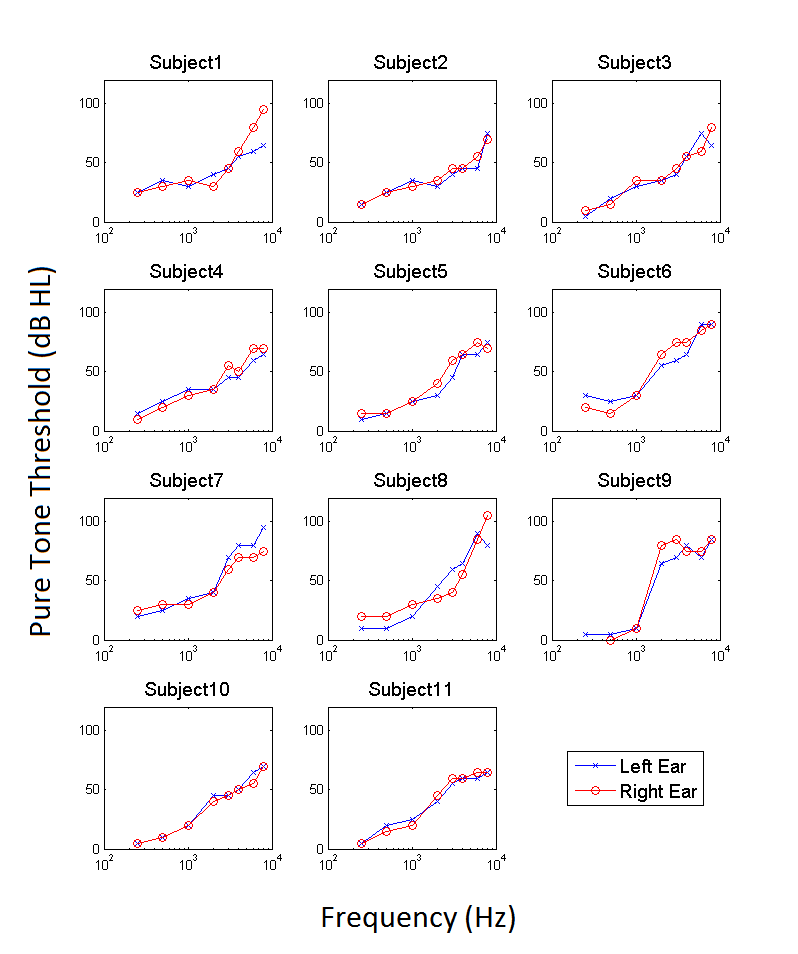
\includegraphics[width=\textwidth]{chap5-audiograms.png}\\
\caption[Audiograms for all subjects]{Audiograms for all subjects.  Right ear is plotted in red o's, left ear in blue x's.  All subjects had mild or moderate symmetrical sensorineural hearing losses.}
\label{ch5-audiograms}
\end{center}
\end{figure}

\subsection{Real Ear Measurements (REMs)}
\paragraph{}REMs provide an illustration of how much gain is being delivered at the ear drum by the hearing instrument, in response to a particular sound sample.  In order to get an idea of the amount of gain being delivered by the NC and WDRC hearing aids, to help interpret the results of the experiment more accurately, REMs were collected at the end of the study for only some participants, due to time and resource constraints.  Typically, REMs are obtained on the person who is fit with hearing aids, in order to verify the amount of gain being delivered by the hearing aids.  We did not have the resources at McMaster to perform these measurements while participants were enlisted in the study, so the measurements were instead performed on the author of this thesis while he wore hearing aids set to the same loss configuration and adjustments that study participants received (using the save files of participants on the fitting software).  A qualified HIS administered the REM procedure at HearAtLast in Burlington, Ontario, using a Medrx Avant system.  Figures 5.3 and 5.4 show real-ear insertion gain (REIG) for two subjects in the study, for WDRC (green curve) and for the NC (blue curve), for the left ear only.  For these subjects, gain was fairly equal between the ears for both the NC and WDRC (right ear not shown).  Another subject's REMs for the left ear are shown in Figure 5.5, with WDRC (blue curve) and the NC (green curve).  For this subject, asymmetric gain was given between the left and right ears for the NC, but not WDRC.  REMs were obtained using ICRA noise as the sound sample, presented at 65 dB SPL.  The spectrum of the ICRA noise is plotted in Figure 5.6.

\begin{figure}[htp]
\begin{center}
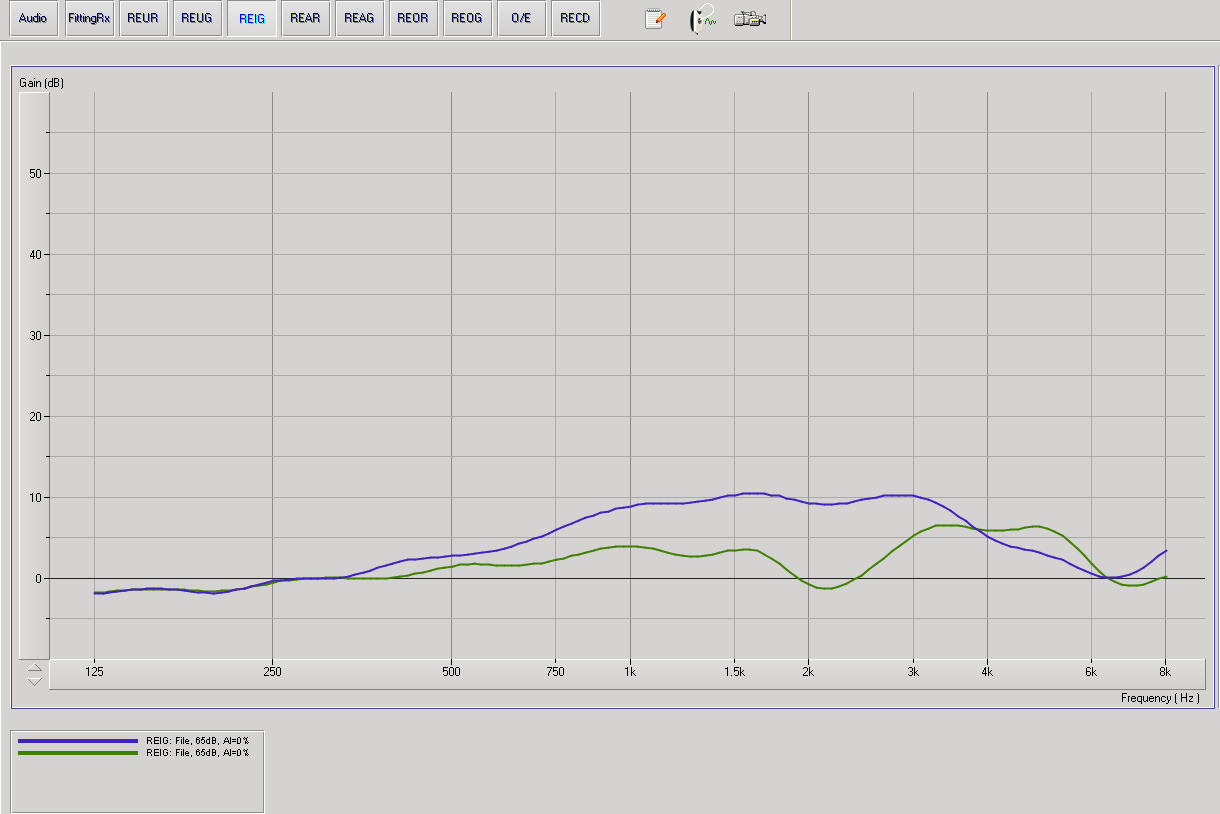
\includegraphics[width=\textwidth]{chap5-reig-walterL.png}\\
\caption[NCStudy2 insertion gain for subject 04]{Insertion gain for subject 04.  Only the left ear is plotted.  Frequency is plotted on the x-axis, and insertion gain on the y-axis.  NC insertion gain is plotted in blue, and WDRC insertion gain is plotted in green.  More gain was being delivered overall with the NC.}
\label{ch5-reig-walterL}
\end{center}
\end{figure}

\begin{figure}[htp]
\begin{center}
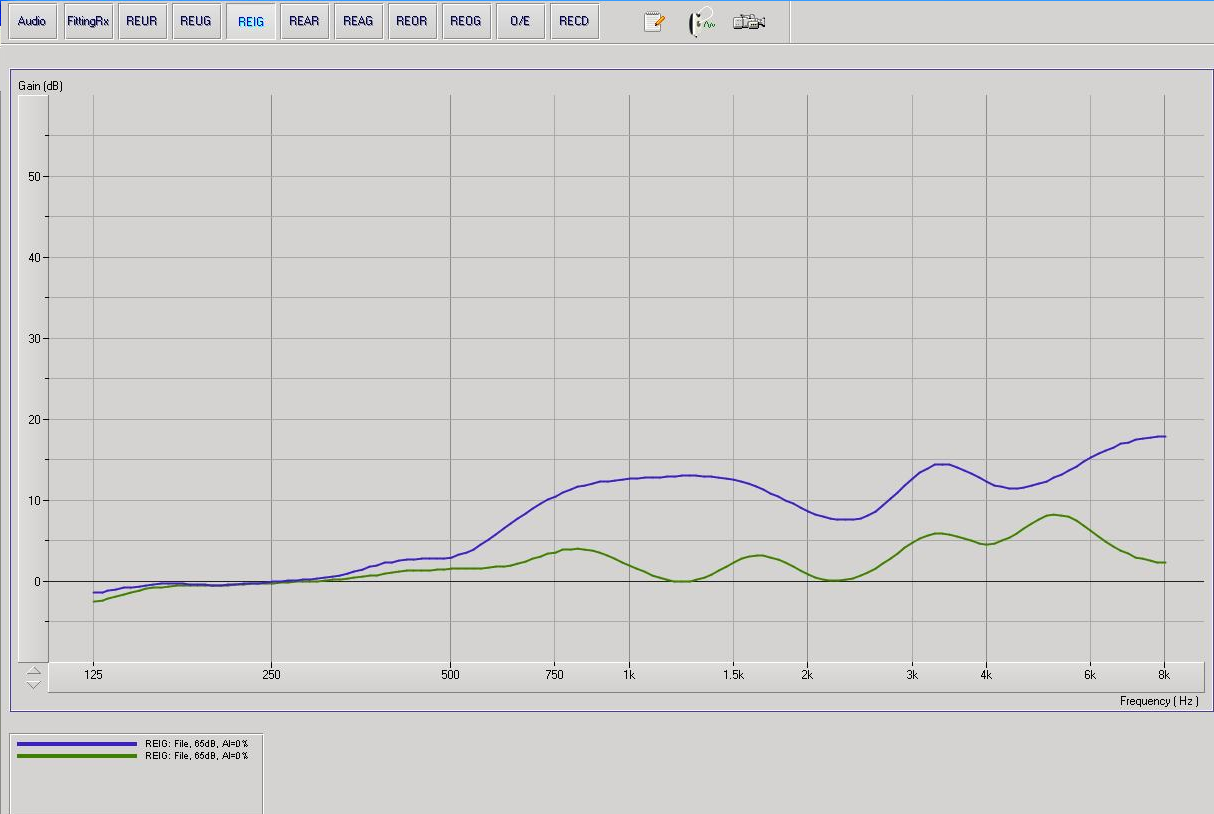
\includegraphics[width=\textwidth]{chap5-reig-dunstanL.png}\\
\caption[NCStudy2 insertion gain for subject 10]{Insertion gain for subject 10.  Only the left ear is plotted.  Frequency is plotted on the x-axis, and insertion gain on the y-axis.  NC insertion gain is plotted in blue, and WDRC insertion gain is plotted in green.  More gain was being delivered overall with the NC.}
\label{ch5-reig-dunstanL}
\end{center}
\end{figure}

\begin{figure}[htp]
\begin{center}
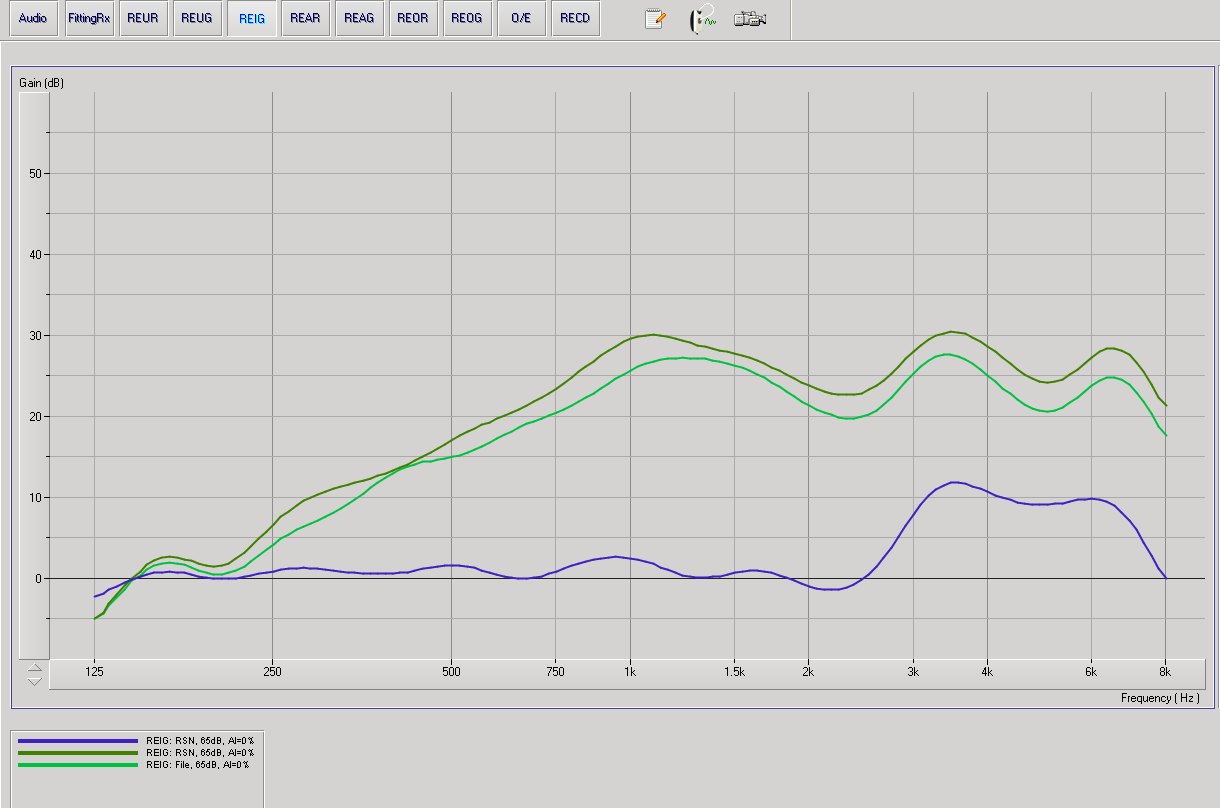
\includegraphics[width=\textwidth]{chap5-reig-anneL.png}\\
\caption[NCStudy2 insertion gain for subject 03]{Insertion gain for subject 03.  Only the left ear is plotted.  Frequency is plotted on the x-axis, and insertion gain on the y-axis.  NC insertion gain is plotted in green (one green curve for ICRA noise, another for speech-shaped noise), and WDRC insertion gain is plotted in blue.  Much more gain was being delivered overall with the NC, and there was asymmetric gain between the ears for the NC (right ear is not shown).}
\label{ch5-reig-anneL}
\end{center}
\end{figure}

\begin{figure}[htp]
\begin{center}
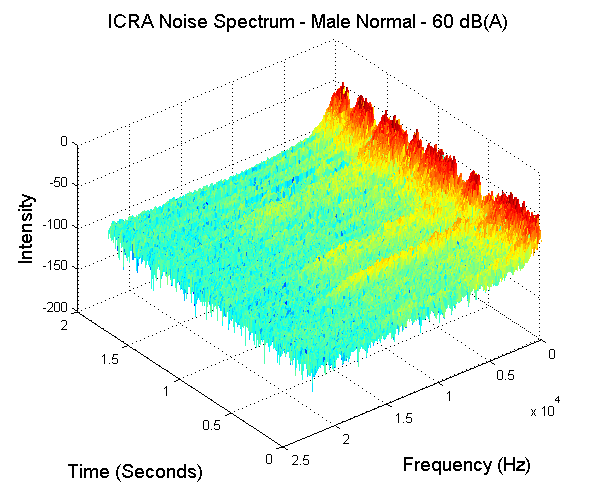
\includegraphics[width=\textwidth]{chap5-ICRA-male-3-band-60-dB.png}\\
\caption[ICRA noise spectrum - 1 male speaker 60 dB(A)]{ICRA noise spectrum - 1 male speaker 60 dB(A).  Similar to other speech shaped noise, most of the acoustic energy for this noise is contained in the lower frequencies, and the noise has speech-like temporal variations as well.}
\label{ch5-ICRAspectrum}
\end{center}
\end{figure}

As you can see, overall, the NC was providing significantly more gain than the WDRC hearing aids, at least for the ICRA stimulus.  In particular, the NC provided much more low-mid frequency gain than the WDRC hearing aids.  Due to the nature of the NC, which adjusts gain dynamically in each frequency channel based on the amount of power, not only in its own frequency channel (WDRC does this), but other channels as well (WDRC does not do this), the real ear measurements taken here may be misleading.  The ICRA stimulus is shaped to have similar spectrotemporal characteristics of speech, but its short term spectrum does not exactly resemble that of speech.  Thus, a more informative approach to validating the gain of the NC hearing aids might be to present real speech.  However, the real ear measurements taken for these three participants' hearing aid fittings does provide evidence that the NC may be providing too much gain in the low frequencies for some non-speech stimuli and some fittings.  In noise, which is often lower frequency, the result may be that the noise is overamplified, masking cues in the higher frequencies which are very important for speech intelligibility.  The evidence is consistent with freeform feedback we received from participants throughout the course of the study, who reported that noise seems to be overamplified with the NC.

\section{Procedures Modified from NCStudy1}
\paragraph{}NCStudy2 used exactly the same procedures and room setup as specified in NCStudy1, with some minor changes.  This section summarizes all of these changes.  If no changes are reported for a given task, it means its procedure was not modified.

\subsection{Hearing In Noise Test (HINT)}
\paragraph{}The length of the HINT task was increased, in order to improve the accuracy of SRT measurements.  Instead of presenting 2 lists of 10 sentences for each hearing aid type, 4 lists of 10 sentences were presented.  2 sets of lists were created (lists 2-5, and lists 6-9), and were used to estimate SRTs.  The use of each set of lists was counterbalanced across hearing aid type, and counterbalanced for the order in which the sets of lists was presented across participants.

\subsection{Word Recognition}
\paragraph{}A word recognition task was added, with the purpose of gauging unaided and aided speech understanding in quiet.  Such an objective measure is used in the audiology profession in order to assess whether the hearing aids provide any real speech intelligibility benefit in quiet.

Two lists were used (Auditec NU6 word lists), and they were always presented in the same order (list 1 for unaided, list 2 for aided).  List 1 had 49 words, and list 2 had 50 words.  The experimenter sat in the testing room with the touchscreen on his/her lap, and initiated each trial by pressing a button on the touchscreen, while the subject was asked to face the center speaker.  On each trial, a word was played from the loudspeaker directly in front of the participant (same room setup as the HINT), and the participant was tasked with repeating the word that they heard.  The experimenter (who had no hearing loss) coded the responses of participants as correct, or incorrect.  The words were calibrated to an overall level of 65 dB SPL.

\subsection{hVd}
\paragraph{}Due to ceiling effects on this task for some participants in NCStudy1, the hVd task was made more difficult for NCStudy2.  In NCStudy1, there was a quiet and a noise (+5 SNR) condition.  In NCStudy2, the quiet condition was modified to include noise (+7 SNR, noise level of 60.5 dB(A)), and the noise condition was made more difficult (+2 SNR, noise level of 65.5 dB(A)).  The rest of the procedure was identical to that used in NCStudy1.

\subsection{APHAB}
\paragraph{}In NCStudy1, participants filled out Form A of the APHAB electronically, whereas participants in NCStudy2 filled out a paper version.  The software only allowed printouts of graphs, as opposed to access to the raw data, and thus the change was made to paper.

The APHAB was administered 3 times in NCStudy2.  The first administration took place on the day participants were fit with their first set of hearing aids, and they were asked to fill out only the unaided portion of Form A immediately before they were fit with hearing aids.  The second occasion where participants filled out the APHAB was during the second test session for the first set of hearing aids, where participants were asked to fill out only the aided portion of Form A.  The last administration took place during the second test session for the second set of hearing aids, and again, participants were asked to only fill out the aided portion of Form A.

\section{Results}
\paragraph{}Analyses for all experiments were performed in R \cite{R2013}.  Where appropriate, the Huynh-Feldt correction for deviations from sphericity ($\tilde{\epsilon}$) was used to compute p values from F tests on within-subjects factors \cite{Maxwell2004}.  In data tables, degrees of freedom and sums of squares for both the numerator (effect of interest) and denominator (error) are reported, along with F and p values, and a measure of effect size, generalized eta squared (abbreviated \emph{ges}).

\subsection{Speech Intelligibility Results}
\subsubsection{Hearing In Noise Test (HINT)}
\paragraph{}SRT estimates for NCStudy2 were computed slightly differently than those for NCStudy1, due to the increased number of sentences presented for NCStudy2.  Instead of averaging the levels of the last 16 sentences, the levels of the last 36 sentences were averaged to estimate SRTs.  A within-subjects ANOVA with a 2-level factor (hearing aid) was performed, with SRT as the dependent measure.  There was no significant effect of hearing aid (F(1,10) = 1.71, p = 0.220).  Group means and standard errors are plotted in Figure 5.7, and individual SRT means and standard deviations are plotted in Figure 5.8.  Individual differences in speech intelligibility in noise were far greater than any difference between the two hearing aids.

%HINT effects of list, HA, session
%\begin{table}[h]
%\begin{tabular}{lrrrrrrrr}
%Effect & DFn & DFd & SSn & SSd & F & p & p<.05 & ges \\
%\hline
%HA &  1 & 10 & 0.90 & 5.24 & 1.71 & 0.220 &   &   0.012 \\
%session &  1 & 10 & 2.91 & 3.23 & 9.01 & 0.013  &   * & 0.474 \\
%list  & 1 & 10 & 0.20 & 5.94 & 0.34 & 0.572 &    &  0.033 \\
%\hline
%\end{tabular}
%\caption{Separate Within-Subjects ANOVAs for HINT Factors}
%\end{table}

\begin{figure}[htp]
\begin{center}
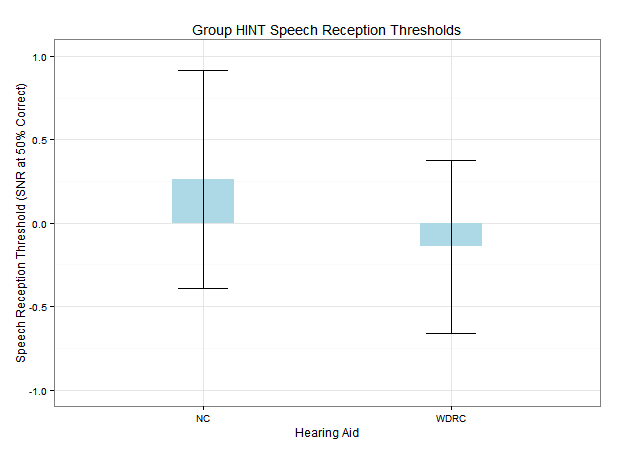
\includegraphics[height=3in]{chap5-hint-group.png} \\
\caption[NCStudy2 group results on the HINT]{NCStudy2 group results on the HINT.  Error bars represent $\pm$ 1 SEM.  Speech reception thresholds were calculated by subtracting the noise level from the average presentation level of the last 36 sentences presented.  There was no significant difference in performance between the NC and WDRC (F(1,10) = 1.71, p = 0.220).}
\label{ch5-hint-group}
\end{center}
\end{figure}

\begin{figure}[htp]
\begin{center}
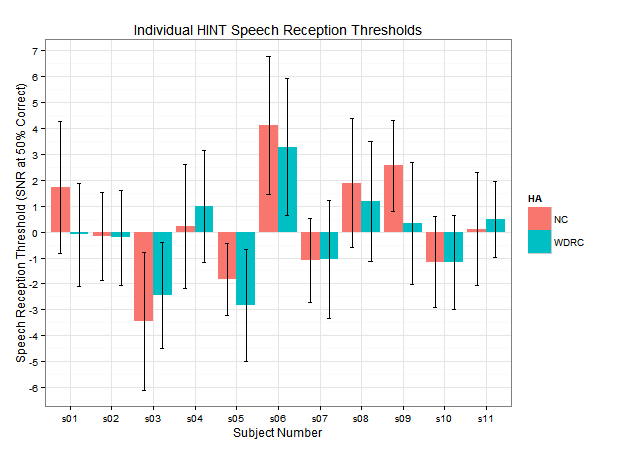
\includegraphics[height=3in]{chap5-hint-indiv.png} \\
\caption[NCStudy2 individual results on the HINT]{NCStudy2 individual results on the HINT.  Error bars represent $\pm$ 1 SD.  Speech reception thresholds were calculated by subtracting the noise level from the average presentation level of the last 36 sentences presented.  Most participants performed approximately equally between NC and WDRC.}
\label{ch5-hint-indiv}
\end{center}
\end{figure}

\subsubsection{Word Recognition}
\paragraph{}A within-subjects ANOVA was performed, with two within-subjects factors, hearing aid (WDRC or NC), and condition (unaided or aided).  The dependent measure was the percentage of words correctly repeated.  The only significant effect was condition (F(1,10) = 38.53, p < 0.001), such that aided performance was superior to unaided performance.  Thus, the use of WDRC or NC hearing aids improved speech intelligibility in quiet.  Detailed statistical results may be seen in Table 5.1.  Group means and standard errors are plotted in Figure 5.9, and individual means and standard deviations are plotted in Figure 5.10.

%word recognition
\begin{table}[htp]
\begin{center}
\begin{tabular}{lrrrrrrrr}
Effect & DFn & DFd & SSn & SSd & F & p & p<.05 & ges \\
\hline
          HA &  1 & 10 & 26.7 & 177 &  1.51 & 0.248  &   &  0.005 \\
        cond &  1 & 10 & 2480 & 644 & 38.53 & < 0.001  &   *** & 0.298 \\
     HA:cond &  1 & 10 & 0.7 & 195 &  0.04 & 0.849  &     & 0.000 \\
\hline
\end{tabular}
\end{center}
\caption{Word Recognition Within-Subjects ANOVA}
\end{table}

\begin{figure}[htp]
\begin{center}
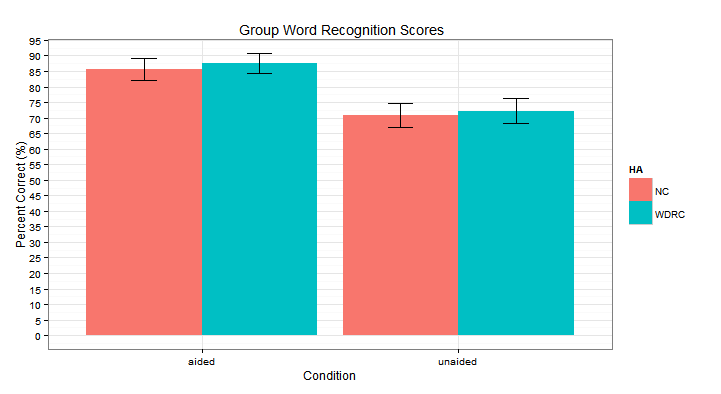
\includegraphics[height=3in]{chap5-wd-group.png} \\
\caption[NCStudy2 group word recognition scores]{NCStudy2 group word recognition scores.  Error bars represent $\pm$ 1 SEM.  There was no significant difference in performance between NC and WDRC (F(1,10) = 1.51, p = 0.248), with each hearing aid conferring approximately a 15\% increase in speech intelligibility performance in quiet.}
\label{ch5-wd-group}
\end{center}
\end{figure}

\begin{figure}[htp]
\begin{center}
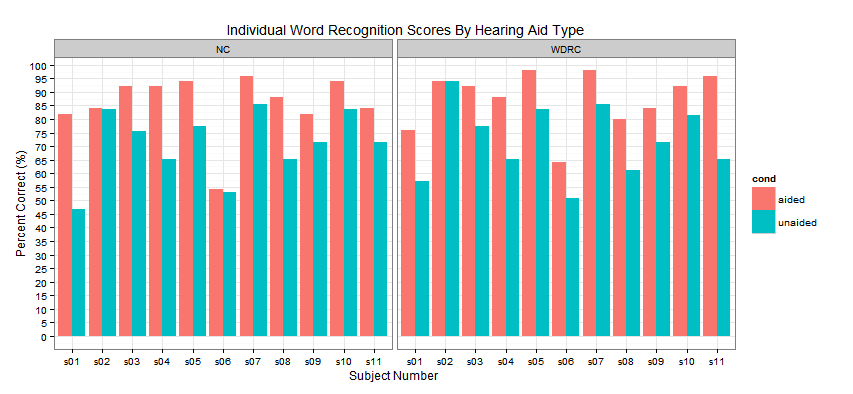
\includegraphics[height=3in]{chap5-wd-indiv.png} \\
\caption[NCStudy2 individual word recognition scores]{NCStudy2 individual word recognition scores.  Most subjects received roughly the same amount of benefit from NC and WDRC.}
\label{ch5-wd-indiv}
\end{center}
\end{figure}

\subsubsection{Consonant Vowel Consonant (CVC)}
\paragraph{}A within-subjects ANOVA was performed, with two within-subjects factors, hearing aid (WDRC or NC), and condition (+7 SNR or +2 SNR).  The dependent measure was the percentage of hVd tokens correctly identified.  The only significant effect was condition (F(1,10) = 26.87, p < 0.001), such that the +2 SNR condition was more difficult than the +7 SNR condition.  Detailed statistical results may be seen in Table 5.2.  Group means and standard errors are plotted in Figure 5.11, and individual means and standard deviations are plotted in Figure 5.12.

\begin{table}[htp]
\begin{center}
\begin{tabular}{lrrrrrrrr}
       Effect & DFn & DFd  &  SSn &  SSd  &    F  &     p & p<.05  &   ges \\
       \hline
          HA &  1 & 10  &   11.7 & 219.5 &   0.54 & 0.481  &     & 0.006 \\
        cond &  1 & 10  &  523.8 & 195.0 &  26.87 & < 0.001  &   *** & 0.199 \\
     HA:cond &  1 & 10  &   23.0 &  88.4 &   2.60 & 0.138  &     & 0.011 \\
     \hline
\end{tabular}
\end{center}
\caption{hVd Within-Subjects ANOVA}
\end{table}

\begin{figure}[htp]
\begin{center}
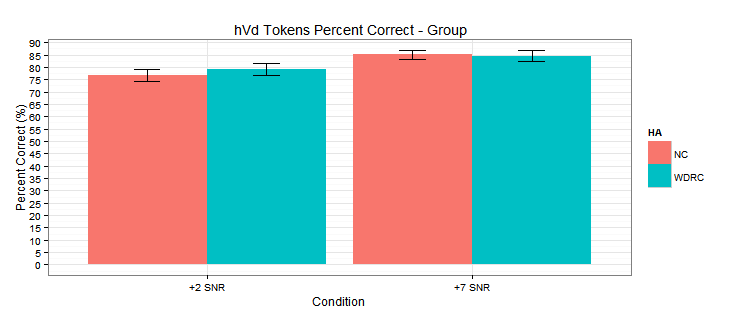
\includegraphics[height=3in]{chap5-hVd-group.png} \\
\caption[NCStudy2 hVd token percent correct - group]{NCStudy2 hVd token percent correct - group.  Error bars represent $\pm$ 1 SEM.  There was no significant difference in performance between NC and WDRC on the percentage of hVd tokens correctly identified (F(1,10) = 0.54, p = 0.481).}
\label{ch5-hVd-group}
\end{center}
\end{figure}

\begin{figure}[htp]
\begin{center}
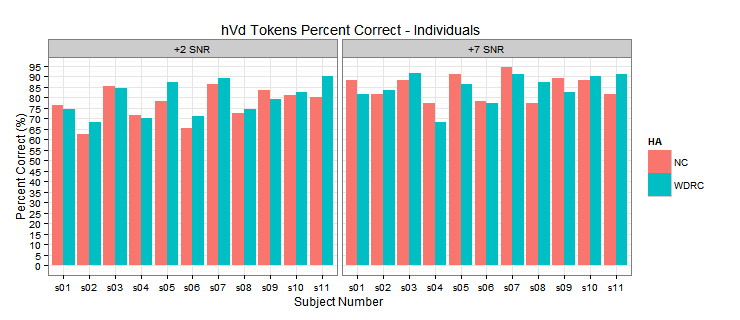
\includegraphics[height=3in]{chap5-hVd-indiv.png} \\
\caption[NCStudy2 hVd token percent correct - individuals]{NCStudy2 hVd token percent correct - individuals.  Some participants correctly identified more hVd tokens with WDRC, while others performed better with NC.}
\label{ch5-hVd-indiv}
\end{center}
\end{figure}

Although there were no significant differences between hearing aids on the overall percentage of hVd tokens correctly identified, there were minor consistent differences between the hearing aids on individual phonemes.  Figure 5.13 plots a confusion matrix both for NC and WDRC averaged over both noise conditions, to illustrate the difficulty of individual phonemes in the experiment.  Figure 5.14 plots the difference between the NC and WDRC confusion matrices for both the +7 SNR and +2 SNR conditions.

\begin{figure}[htp]
\begin{center}
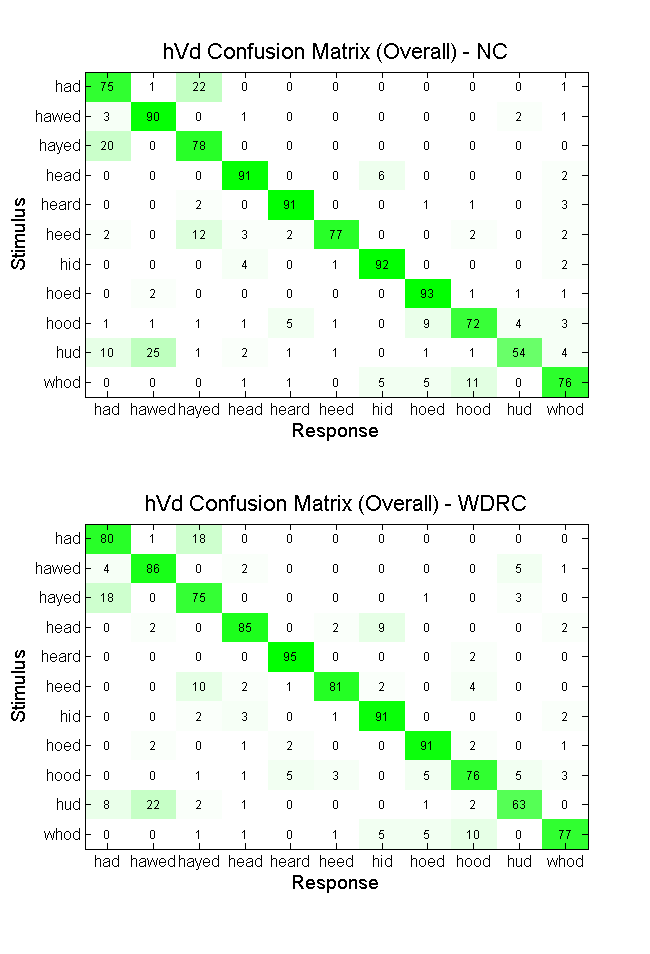
\includegraphics[height=7in]{chap5-hVd-ovr.png} \\
\caption[NCStudy2 hVd overall confusion matrices]{hVd confusion matrices.  Data shown are for the noise and quiet conditions amalgamated together.  \emph{Top}: hVd confusion matrix for NC.  \emph{Bottom}: hVd confusion matrix for WDRC.  For many of the syllables, performance is at near ceiling.  Few differences exist between NC and WDRC; the syllables where WDRC and NC differ the most are /head/, and /hud/. }
\label{ch5-hVd-ovr}
\end{center}
\end{figure}

\clearpage

\begin{figure}[htp]
\begin{center}
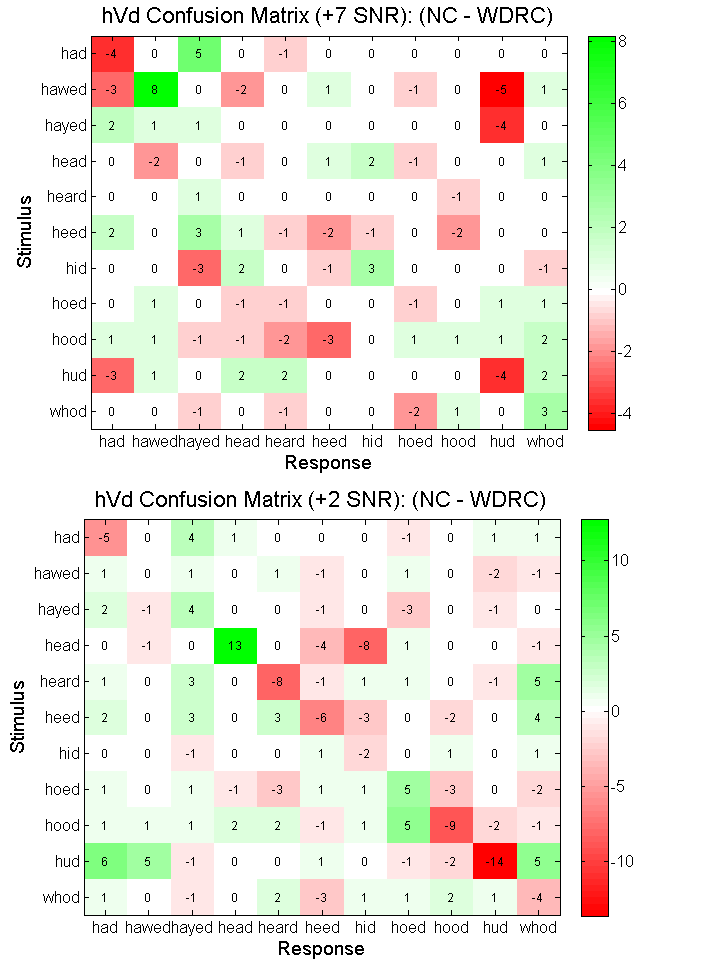
\includegraphics[height=7in]{chap5-hVd-cond-difference.png} \\
\caption[NCStudy2 difference between hVd confusion matrices (NC - WDRC)]{NCStudy2 difference between hVd confusion matrices (NC - WDRC).  \emph{Top:} Difference between hVd confusion matrices for the +7 SNR condition.  \emph{Bottom:} Difference between hVd confusion matrices for the +2 SNR condition.  Each tile represents NC \% response - WDRC \% response.  Differences between NC and WDRC are accentuated in the noisier condition; in noise, NC restores /head/ better than WDRC, while WDRC restores mainly /hud/ better.}
\label{ch5-hVd-cond-difference}
\end{center}
\end{figure}

\subsubsection{Vowel Consonant Vowel (VCV)}
\paragraph{}A within-subjects ANOVA was performed, with two within-subjects factors, hearing aid (WDRC or NC), and condition (quiet or noise).  The dependent measure was the percentage of VCV tokens correctly identified.  There were two significant main effects; a main effect of condition (F(1,10) = 477.44, p < 0.001), such that the noise condition was much more difficult than the quiet condition, and hearing aid (F(1,10) = 10.55, p = 0.009), such that WDRC outperformed the NC.  Detailed statistical results may be seen in Table 5.3.  Group means and standard errors are plotted in Figure 5.15, and individual means and standard deviations are plotted in Figure 5.16.

\begin{table}[htp]
\begin{center}
\begin{tabular}{lrrrrrrrr}
       Effect & DFn & DFd  &  SSn &  SSd  &    F  &     p & p<.05  &   ges \\
       \hline
          HA &  1 & 10 & 289 & 274 & 10.55 & 0.009 &    ** & 0.088 \\
        cond &  1 & 10 & 13800 & 289 & 477.44 & < 0.001 &    *** & 0.821 \\
     HA:cond &  1 & 10 & 7 & 137 &  0.51 & 0.493  &     & 0.002 \\
     \hline
\end{tabular}
\end{center}
\caption{VCV Within-Subjects ANOVA}
\end{table}

\begin{figure}[htp]
\begin{center}
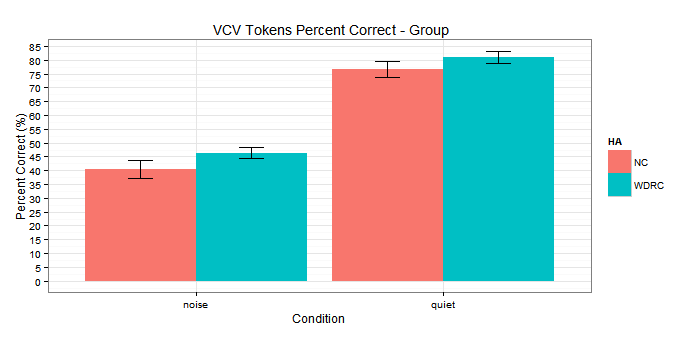
\includegraphics[height=3in]{chap5-vcv-group.png} \\
\caption[NCStudy2 VCV token percent correct - group]{NCStudy2 VCV token percent correct - group.  Error bars represent $\pm$ 1 SEM.  There was a significant difference in performance between NC and WDRC on the percentage of VCV tokens correctly identified (F(1,10) = 10.55, p = 0.009).}
\label{ch5-vcv-group}
\end{center}
\end{figure}

\begin{figure}[htp]
\begin{center}
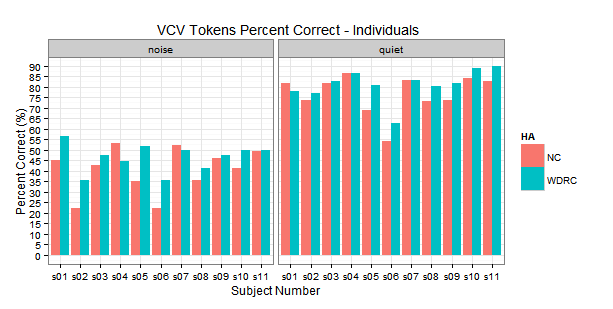
\includegraphics[height=3in]{chap5-vcv-indiv.png} \\
\caption[NCStudy2 VCV token percent correct - individuals]{NCStudy2 VCV token percent correct - individuals.  The main effect of hearing aid was not simply driven by a few participants performing better with WDRC hearing aids.  There were only 2 participants out of 11 who identified more tokens correctly with the NC in noise, and only 1 out of 11 in quiet.}
\label{ch5-vcv-indiv}
\end{center}
\end{figure}

There were consistent differences between the hearing aids on individual phonemes.  Figure 5.17 plots a confusion matrix both for NC and WDRC averaged over both conditions, to illustrate the difficulty of individual phonemes in the experiment.  Figure 5.18 plots the difference between the NC and WDRC confusion matrices for both the quiet and noise conditions.

\begin{figure}[htp]
\begin{center}
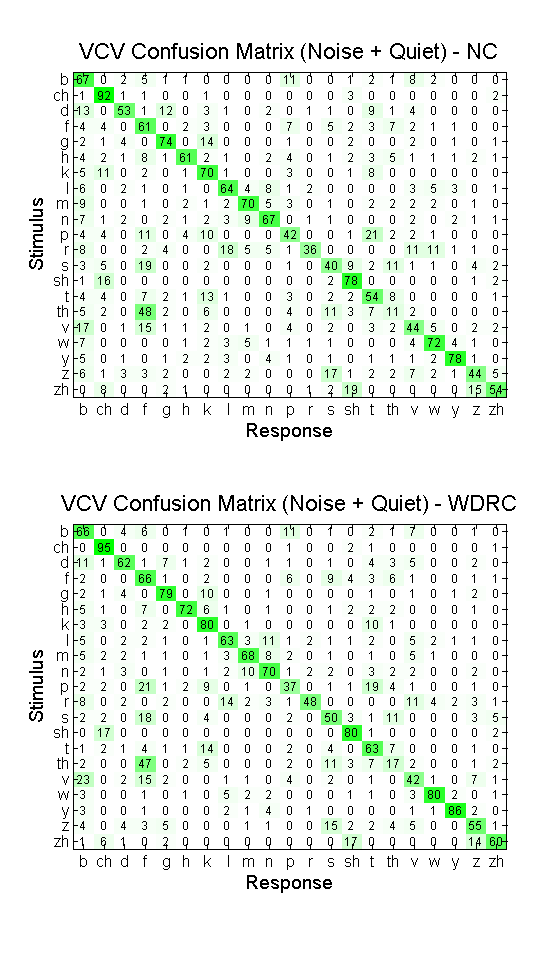
\includegraphics[height=7in]{chap5-VCV-ovr.png} \\
\caption[NCStudy2 VCV overall confusion matrices]{NCStudy2 VCV confusion matrices.  Data shown are for the noise and quiet conditions amalgamated together.  \emph{Top}: VCV confusion matrix for NC.  \emph{Bottom}: VCV confusion matrix for WDRC.}
\label{ch5-VCV-ovr}
\end{center}
\end{figure}

\clearpage

\begin{figure}[htp]
\begin{center}
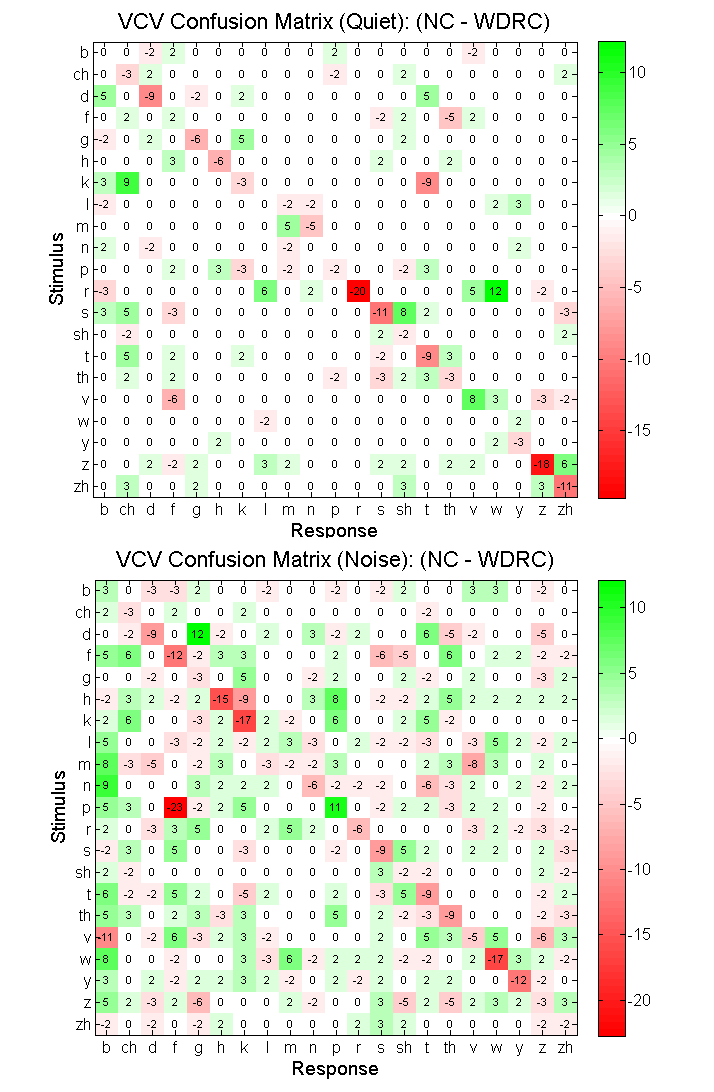
\includegraphics[height=7in]{chap5-VCV-cond-difference.png} \\
\caption[NCStudy2 difference between VCV confusion matrices (NC - WDRC) ]{NCStudy2 difference between VCV confusion matrices (NC - WDRC).  \emph{Top:} Difference between VCV confusion matrices for the quiet condition.  \emph{Bottom:} Difference between VCV confusion matrices for the noise condition.  Most of the consonants were restored better with WDRC.}
\label{ch5-VCV-cond-difference}
\end{center}
\end{figure}

\subsection{Music Perception Results}
\subsubsection{Mistuned Harmonic}
\paragraph{}A within-subjects ANOVA was performed, with two within-subjects factors, hearing aid (WDRC or NC), and tone (200 Hz or 600 Hz).  The dependent measure was the mistuned harmonic threshold.  The only significant effect was a main effect of tone (F(1,10) = 5.00, p = 0.049), such that the higher complex tone (600 Hz) was more difficult than the lower complex tone (200 Hz).  Detailed statistical results may be seen in Table 5.4.  Group means and standard errors are plotted in Figure 5.19, and individual means and standard deviations are plotted in Figure 5.20.

\begin{table}[htp]
\begin{center}
\begin{tabular}{lrrrrrrrr}
       Effect & DFn & DFd  &  SSn &  SSd  &    F  &     p & p<.05  &   ges \\
       \hline
          HA &  1 & 10 &  21 & 139 & 1.53 & 0.245 &      & 0.019 \\
        tone &  1 & 10 & 229 & 459 & 5.00 & 0.049 &    * & 0.170 \\
     HA:tone &  1 & 10 &   1 & 165 & 0.03 & 0.859 &      & 0.000 \\
     \hline
\end{tabular}
\end{center}
\caption{Mistuned Harmonic Within-Subjects Factorial ANOVA}
\end{table}

\begin{figure}[htp]
\begin{center}
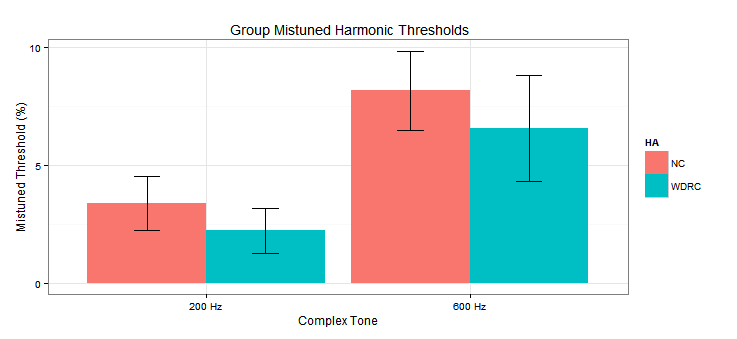
\includegraphics[height=3in]{chap5-mhn-group.png} \\
\caption[NCStudy2 mistuned harmonic - group thresholds]{NCStudy2 mistuned harmonic - group results.  Error bars represent $\pm$ 1 SEM.  There was no significant difference between NC and WDRC (F(1,10) = 1.53, p = 0.245), but the higher frequency complex tone was significantly more difficult (F(1,10) = 5.00, p = 0.049).}
\label{chap5-mhn-group}
\end{center}
\end{figure}

\begin{figure}[htp]
\begin{center}
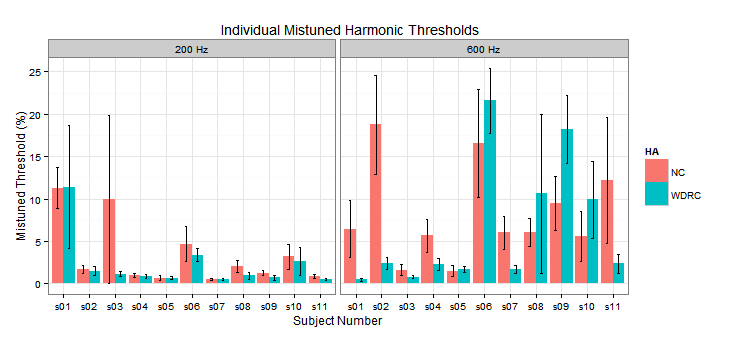
\includegraphics[height=3in]{chap5-mhn-indiv.png} \\
\caption[NCStudy2 mistuned harmonic - individual thresholds]{NCStudy2 mistuned harmonic - individual results.  Error bars represent $\pm$ 1 SD.  There are huge individual differences on this task.}
\label{chap5-mhn-indiv}
\end{center}
\end{figure}

\subsubsection{Timbre Perception}
\paragraph{}A within-subjects ANOVA was performed, with two within-subjects factors, hearing aid (WDRC or NC), and harmonic (fundamental or second harmonic).  The dependent measure was the harmonic intensity threshold.  The only significant effect was a main effect of harmonic (F(1,10) = 47.34, p < 0.001), such that participants were more sensitive to changes in intensity of the fundamental than the second harmonic.  Detailed statistical results may be seen in Table 5.5.  Group means and standard errors are plotted in Figure 5.21, and individual means and standard deviations are plotted in Figure 5.22.

\begin{table}[htp]
\begin{center}
\begin{tabular}{lrrrrrrrr}
       Effect & DFn & DFd  &  SSn &  SSd  &    F  &     p & p<.05  &   ges
       \\
       \hline
          HA &  1 & 10 &    59 & 1822 &  0.32 & 0.583  &     & 0.008 \\
        harm &  1 & 10 &  6299 & 1330 & 47.34 & < 0.001 &    *** & 0.456 \\
     HA:harm &  1 & 10 &    57 & 730  & 0.78 & 0.399    &   & 0.007 \\
     \hline
\end{tabular}
\end{center}
\caption{Timbre Perception Within-Subjects Factorial ANOVA}
\end{table}

\begin{figure}[htp]
\begin{center}
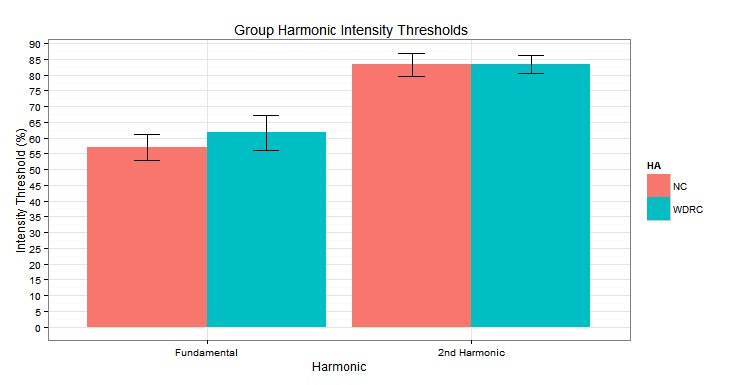
\includegraphics[height=2.5in]{chap5-timbre-group.png} \\
\caption[NCStudy2 timbre perception - group thresholds]{NCStudy2 timbre perception - group thresholds.  Error bars represent $\pm$ 1 SEM.  There was no significant difference between NC and WDRC (F(1,10) = 0.32, p = 0.583), but the fundamental was easier to discriminate than the second harmonic (F(1,10) = 47.34, p < 0.001).}
\label{chap5-timbre-group}
\end{center}
\end{figure}

\begin{figure}[htp]
\begin{center}
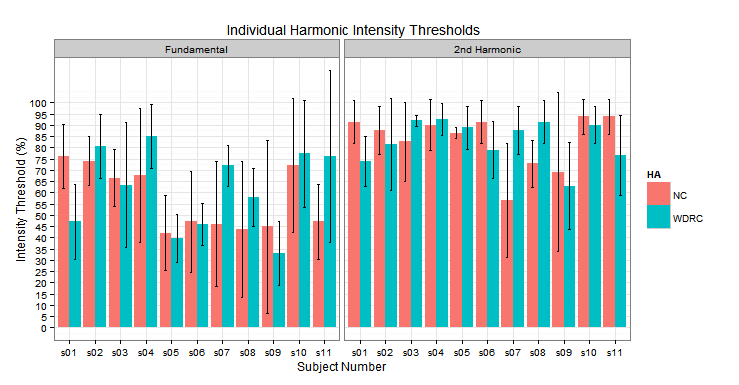
\includegraphics[height=2.5in]{chap5-timbre-indiv.png} \\
\caption[NCStudy2 timbre perception - individual thresholds]{NCStudy2 timbre perception - individual thresholds.  Error bars represent $\pm$ 1 SD.}
\label{chap5-timbre-indiv}
\end{center}
\end{figure}

\subsubsection{Gap Detection}
\paragraph{}A within-subjects ANOVA was performed, with hearing aid (WDRC or NC) as the only factor.  The dependent measure was the gap threshold.  There was a main effect of hearing aid (F(1,10) = 18.1, p = 0.002), such that participants could detect a smaller silent gap in a sound while wearing WDRC.  Detailed statistical results may be seen in Table 5.6.  Group means and standard errors are plotted in Figure 5.23, and individual means and standard deviations are plotted in Figure 5.24.

\begin{table}[htp]
\begin{center}
\begin{tabular}{lrrrrrrrr}
       Effect & DFn & DFd  &  SSn &  SSd  &    F  &     p & p<.05  &   ges
       \\
       \hline
          HA &  1 & 10  & 566 & 314 & 18.1 & 0.002   &  ** & 0.343 \\
      \hline
\end{tabular}
\end{center}
\caption{Gap Detection Within-Subjects ANOVA}
\end{table}

\begin{figure}[htp]
\begin{center}
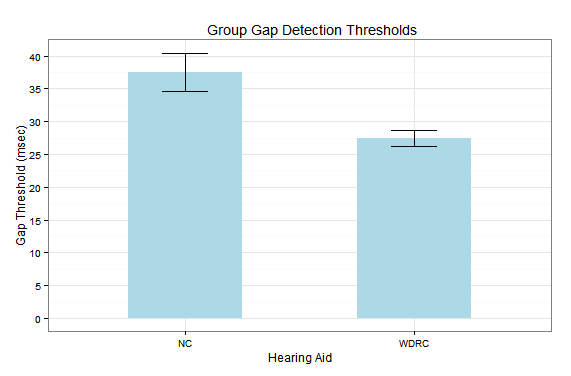
\includegraphics[height=3in]{chap5-gap-group.png} \\
\caption[NCStudy2 gap detection - group thresholds]{NCStudy2 gap detection - group thresholds.  Error bars represent $\pm$ 1 SEM.  Performance on the task was significantly better with WDRC than NC, as determined with a within-subjects ANOVA (F(1,10) = 18.1, p = 0.002).}
\label{chap5-gap-group}
\end{center}
\end{figure}

\begin{figure}[htp]
\begin{center}
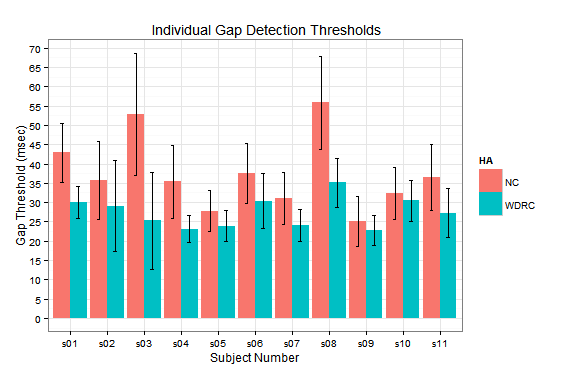
\includegraphics[height=3in]{chap5-gap-indiv.png} \\
\caption[NCStudy2 gap detection - individual thresholds]{NCStudy2 gap detection - individual thresholds.  Error bars represent $\pm$ 1 SD.  All 11 participants performed better on the task with WDRC.}
\label{chap5-gap-indiv}
\end{center}
\end{figure}

\subsection{Sound Localization Results}
\paragraph{}A within-subjects ANOVA was performed, with three within-subjects factors, hearing aid (WDRC or NC), stimulus (low freq, high freq, or phone), and angle (0 to 90$^\circ$ in 15$^\circ$ increments).  The dependent measure was the error (|Stimulus$^\circ$ - Response$^\circ$|).  After correcting for deviations from sphericity with the Huynh-Feldt correction factor ($\tilde{\epsilon}$), the only significant effect was a main effect of stimulus (F(2,20) = 121.64, p < 0.001, $\tilde{\epsilon}$ = 0.643), such that the high frequency stimulus was much more difficult than the phone or low frequency stimuli.  There was also a trending main effect of angle (F(6,60) = 2.75, p = 0.098, $\tilde{\epsilon}$ = 0.287), and a trending interaction of stimulus and angle (F(12,120) = 2.57, p = 0.093, $\tilde{\epsilon}$ = 0.188).  Detailed statistical results may be seen in Table 5.7.  Group means and standard errors are plotted, as a function of stimulus in Figure 5.25, as a function of angle in Figure 5.26, and combined in Figure 5.27.  Figure 5.28 also shows the distribution of responses on each condition for both NC and WDRC.

\begin{table}[htp]
\begin{tabular}{lrrrrrrrr}
\hline
ANOVA & & & & & & & & \\
         Effect & DFn & DFd  &    SSn &  SSd   &     F   &  p & p<.05  &  ges \\
            HA &  1 & 10  &  69 & 1621 &  0.42 & 0.530    &   & 0.002 \\
          stim &  2 & 20 & 28876 & 2374 & 121.64 & < 0.001  &  *** & 0.469 \\
         angle &  6 & 60 & 2321 & 8450 &  2.75 & 0.020   &  * & 0.066 \\
       HA:stim &  2 & 20 &  160 & 2271 &  0.70 & 0.506  &    & 0.005 \\
      HA:angle &  6 & 60  &  95 & 1492 &  0.64 & 0.700   &    & 0.003 \\
    stim:angle & 12 & 120 & 1961 & 7617 &  2.57 & 0.005  &   ** & 0.057 \\
 HA:stim:angle & 12 & 120 &  494 & 3127 &  1.58 & 0.107  &     & 0.015 \\
\hline
\end{tabular}
\begin{tabular}{lrrr}
Mauchly's Test for Sphericity & & & \\
      Effect  &      W   &     p & p<.05 \\
       stim & 0.347 & 0.009 &     ** \\
      angle & < 0.001 & < 0.001 &     *** \\
    HA:stim & 0.242 & 0.002 &     ** \\
   HA:angle & 0.031 & 0.170 &       \\
 stim:angle & < 0.001 & < 0.001 &     *** \\
\hline
\end{tabular}
\begin{tabular}{lrrrrrr}
Sphericity Corrections & & & & & & \\
         Effect &  GGe &   p[GG] & p[GG]<.05 &   HFe  &   p[HF] & p[HF]<.05 \\
          stim & 0.605 & < 0.001 &         *** & 0.643 & < 0.001 &  *** \\
         angle & 0.251 & 0.107 &           & 0.287 & 0.098 &  . \\
       HA:stim & 0.569 & 0.437 &           & 0.593 & 0.442 &    \\
      HA:angle & 0.466 & 0.587 &           & 0.664 & 0.639 &    \\
    stim:angle & 0.154 & 0.106 &           & 0.188 & 0.093 &  .  \\
 HA:stim:angle & 0.267 & 0.212 &           & 0.409 & 0.185 &    \\
\hline
\end{tabular}
\caption{Sound Localization Within-Subjects ANOVA}
\end{table}

\begin{figure}[htp]
\begin{center}
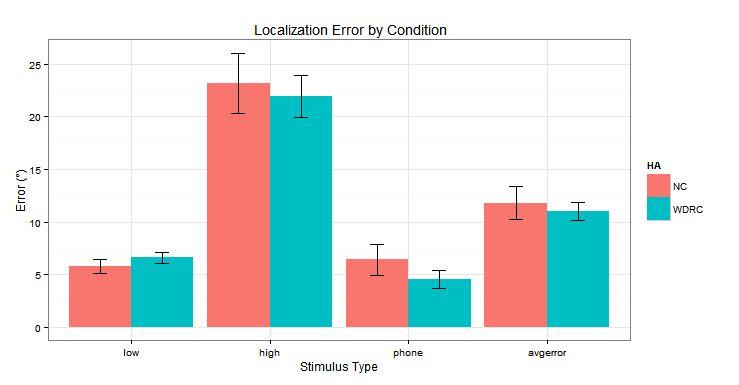
\includegraphics[height=3in]{chap5-loc-cond.png} \\
\caption[NCStudy2 sound localization results - stimulus type]{NCStudy2 sound localization results - stimulus type.  Error bars represent $\pm$ 1 SEM.  There was a main effect of stimulus type (F(2,20) = 121.64, p < 0.001, $\tilde{\epsilon}$ = 0.643), such that the higher frequency sound was more difficult to localize.}
\label{chap5-loc-cond}
\end{center}
\end{figure}

\begin{figure}[htp]
\begin{center}
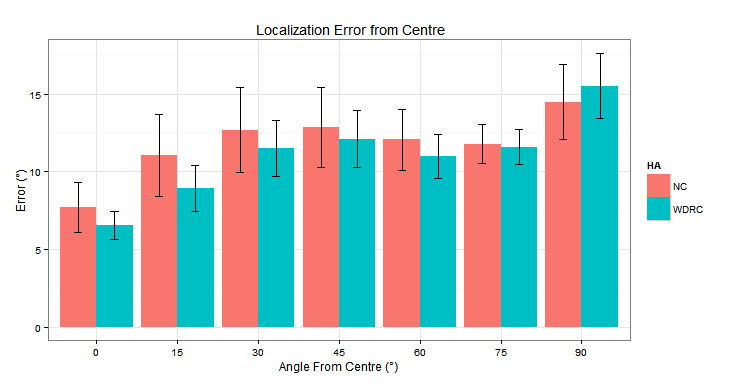
\includegraphics[height=3in]{chap5-loc-spk.png} \\
\caption[NCStudy2 sound localization results - angle]{NCStudy2 sound localization results - angle.  Error bars represent $\pm$ 1 SEM.  Generally speaking, the further the stimulus is presented from centre, the greater the error.}
\label{chap5-loc-spk}
\end{center}
\end{figure}

\begin{figure}[htp]
\begin{center}
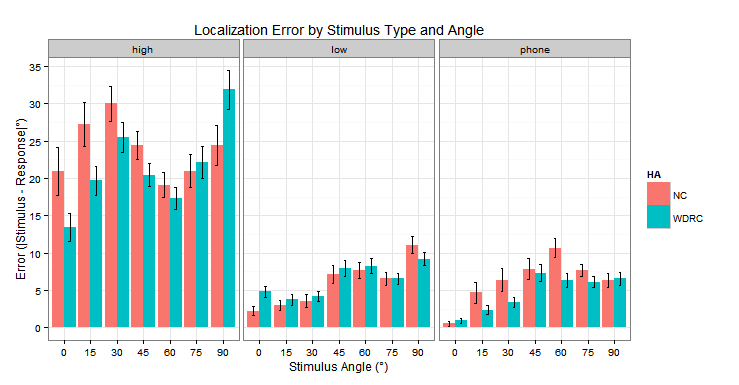
\includegraphics[height=3in]{chap5-loc-cond+spk.png} \\
\caption[NCStudy2 sound localization results - stimulus type and angle]{NCStudy2 sound localization results - stimulus type and angle.  Error bars represent $\pm$ 1 SEM.}
\label{chap5-loc-cond-spk}
\end{center}
\end{figure}

\begin{figure}[htp]
\begin{center}
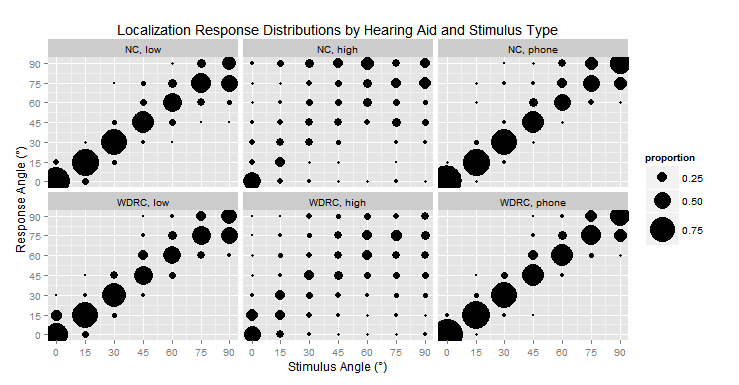
\includegraphics[height=3in]{chap5-loc-prop.png} \\
\caption[NCStudy2 sound localization results - response distributions]{NCStudy2 sound localization response distributions.  Circle area is proportional to number of responses at a particular stimulus, response configuration.}
\label{chap5-loc-cond-prop}
\end{center}
\end{figure}

\subsection{Subjective Measure Results}

\subsubsection{APHAB}
\paragraph{}A within-subjects ANOVA was performed, with two within-subjects factors, hearing aid (WDRC or NC), and APHAB subscale (Ease of Communication, Reverberation, Background Noise, Aversiveness of Sounds).  The dependent measure was the average score from 1-7 on each subscale.  Group means and standard errors are plotted as a function of subscale in Figure 5.29.

After correcting for deviations from sphericity with the Huynh-Feldt correction factor ($\tilde{\epsilon}$), all main effects and the interaction were significant (see Table 5.8).  Thus, simple main effects of hearing aid at each level of APHAB subscale were investigated (see Table 5.9 for detailed results).  There was a significant simple main effect of hearing aid for the Aversiveness of Sounds subscale (F(1,10) = 16.20, p = 0.002), such that participants expressed more aversion to sounds while wearing the NC than they did for WDRC, and there was a trending simple main effect of hearing aid for Background Noise (F(1,10) = 3.61, p = 0.087), such that participants expressed more problems with background noise while wearing the NC.  The trending main effect of background noise should be interpreted with caution, as a correction for multiple comparisons was not been applied, and it is only a trend.  It is of the author's opinion that it is worth mentioning, since it is potentially useful for interpretation of the results on the objective tests.

The Aversiveness of Sounds subscale contains items related to overly loud/uncomfortable alarms or bells, traffic noises, running water, construction work, fire engines, and screeching tires.

%APHAB
%figure
\begin{figure}[htp]
\begin{center}
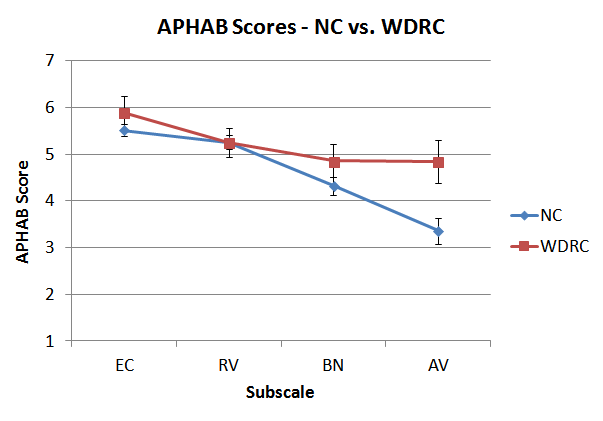
\includegraphics[height=3in]{chap5-aphab-group.png} \\
\caption[NCStudy2 APHAB results]{NCStudy2 APHAB results.  APHAB subscale abbreviations are plotted on the x-axis, corresponding to: Ease of Communication, Reverberation, Background Noise, and Aversiveness of Sounds, respectively.  Lower APHAB scores correspond to more problems.  Error bars represent $\pm$ 1 SEM.  A within-subjects ANOVA indicated that there was an interaction between HA and APHAB subscale (F(3,30) = 6.74, p = 0.005, $\tilde{\epsilon}$ = 0.721).  Simple main effects of HA tested for each APHAB subscale showed that the NC was associated with significantly greater aversion to sounds (F(1,10) = 16.20, p = 0.002).}
\label{chap5-aphab-group}
\end{center}
\end{figure}

\clearpage

%APHAB Within-Subjects ANOVA Table
\begin{table}[htp]
\begin{tabular}{lrrrrrrrr}
  \hline
  ANOVA & & & & & & & & \\
  Effect & DFn & DFd & SSn & SSd & F & p & p<.05 & ges \\
         HA  & 1 & 10 &   7.9 & 10.6 &  7.44  & 0.021  &   * & 0.093 \\
   subscale  & 3 & 30 &  33.3 & 28.9 & 11.52 & < 0.001 &     *** & 0.302 \\
HA:subscale  & 3 & 30 &   6.7 & 9.9 &  6.74 & 0.001  &   ** & 0.080 \\
   \hline
\end{tabular}
\begin{tabular}{lrrr}
  Mauchly's Test for Sphericity & & & \\
  Effect &     W   &     p & p<.05 \\
   subscale & 0.055 & < 0.001 &    *** \\
HA:subscale & 0.329 & 0.087 &      \\
  \hline
\end{tabular}
\begin{tabular}{lrrrrrr}
  Sphericity Corrections & & & & & & \\
   Effect &  GGe &  p[GG] & p[GG]<.05 &  HFe &  p[HF] & p[HF]<.05 \\
   subscale & 0.423 & 0.003 &        ** & 0.457 & 0.003 &        ** \\
HA:subscale & 0.598 & 0.008 &        ** & 0.721 & 0.005 &        ** \\
   \hline
\end{tabular}
\caption{APHAB Within-Subjects Factorial Anova}
\end{table}

%APHAB table-simple main effects
\begin{table}[htp]
\begin{center}
\begin{tabular}{lrrrrrrrr}
Subscale & DFn & DFd & SSn & SSd & F & p & p<.05 & ges \\
\hline
EC &  1 & 10 &  0.79 & 4.70 &  1.68 & 0.224  & &    0.0507 \\
RV &  1 & 10 & 0.00 & 3.91 & 0.00 & 0.965 & & 0.000 \\
BN &  1 & 10 &  1.58 & 4.38 &  3.61 & 0.087 &    . & 0.081 \\
AV &  1 & 10 & 12.20 & 7.50 & 16.20 & 0.002 &    ** & 0.283 \\
\hline
\end{tabular}
\end{center}
\caption{Simple Main Effect of HA for each APHAB Subscale}
\end{table}

\subsubsection{Sound Quality}
\paragraph{}A within-subjects ANOVA was performed, with two within-subjects factors, hearing aid (WDRC or NC), and questionnaire subtype (music or overall).  The dependent measure was a composite score, averaged over all items in each condition for the questionnaire.  The music quality composite score was an average of 4 items, whereas the overall quality composite score was an average of 10 items.  The only significant effect was a main effect of questionnaire subtype (F(1,10) = 13.23, p = 0.005), which is not very interesting.  Detailed statistical results may be seen in Table 5.10.  Group means and standard errors are plotted in Figure 5.30.

%figure
\begin{figure}[htp]
\begin{center}
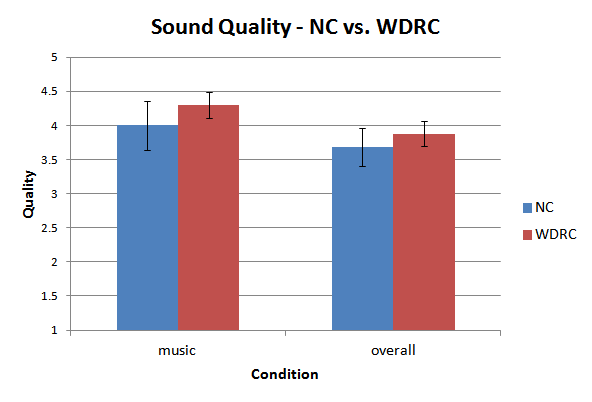
\includegraphics[height=3in]{chap5-qual-group.png} \\
\caption[NCStudy2 sound quality results]{NCStudy2 sound quality results.  Music quality was assessed on a scale of 1-5 on various dimensions (naturalness, pleasantness, fullness, clarity).  For each person and set of hearing aids, a composite score was computed by averaging a participant's scores over all dimensions.  Overall quality was computed by averaging scores over several listening situations, each measured on a scale of 1-5, ranging from unpleasant to pleasant.  Error bars represent $\pm$ 1 SEM.  The listening situations included speech in quiet with one person, speech with several talkers, car radio, telephone, television, small and large music performances, speech/music at the cinema, and favorite recordings of the participant's favorite music.  There were no significant differences between NC and WDRC on sound quality (F(1,10) = 0.50, p = 0.496).}
\label{chap5-qual-group}
\end{center}
\end{figure}

%table
\begin{table}[htp]
\begin{center}
\begin{tabular}{lrrrrrrrr}
Effect & DFn & DFd  &    SSn &  SSd &      F  &      p & p<.05   &   ges \\
\hline
     HA &  1 & 10 &  0.68 & 13.64 &  0.50 & 0.496 &      & 0.022 \\
   cond &  1 & 10 &  1.49 & 1.12  & 13.23 & 0.005 &    ** & 0.047 \\
HA:cond &  1 & 10 &  0.02 & 2.27  & 0.11 & 0.751  &     & 0.001 \\
\hline
\end{tabular}
\end{center}
\caption{Sound Quality Within-Subjects ANOVA}
\end{table}

\subsubsection{Structured Diary}
\paragraph{}To properly analyze the data from the structured diary, since there were three different dependent measures, the data were first split into three separate subsets: one for the loudness of target speech, another for the clarity of speech, and last, for the loudness of background noise.  A within-subjects ANOVA was performed for each subset of data, with two within-subjects factors, hearing aid (WDRC or NC), and listening situation (conversing in a quiet living room, conversing on a car/bus, having a meal with 2-3 people, conversing with a noisy group, listening to someone at a distance, and television at home).  The subset of data for clarity was largely uninteresting, and is ignored here. There were close to significant interactions between hearing aid and listening situation for both the loudness of target speech data (F(5,30) = 2.12, p = 0.13, $\tilde{\epsilon}$ = 0.620) and the loudness of background noise data (F(5,30) = 2.19, p = 0.09, $\tilde{\epsilon}$ = 0.89).  Once again, no corrections for multiple comparisons were made here, so the results must be interpreted with caution.  Figure 5.31 depicts results on each listening situation for the target loudness data, and Figure 5.32 depicts results on each listening situation for the background noise data.

In Figure 5.31, although no statistical analyses were performed, the loudness of target speech for the NC generally seems to louder, and closer to the optimal score (3) than WDRC, particularly in quiet, while watching television, and while having a meal with 2-3 people.

\begin{figure}[htp]
\begin{center}
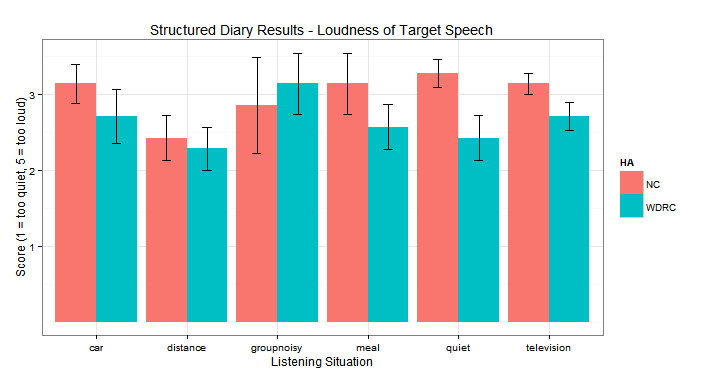
\includegraphics[height=3in]{chap5-structured-targ-speech.png} \\
\caption[NCStudy2 structured diary results - loudness of target speech]{NCStudy2 structured diary results - loudness of target speech.  Error bars represent $\pm$ 1 SEM.  The loudness of target speech for the NC generally seems to louder, and closer to the optimal score (3) than WDRC, particularly in quiet, while watching television, and while having a meal with 2-3 people.}
\label{chap5-struct-back-noise}
\end{center}
\end{figure}

In Figure 5.32, although no statistical analyses were performed, it is quite clear that the greatest difference in background noise ratings between the NC and WDRC is with a group of people in a noisy situation.  Participants tend to report that the loudness of background noise is too loud with the NC for this particular situation, while for the other situations there are no differences between the NC and WDRC.

\begin{figure}[htp]
\begin{center}
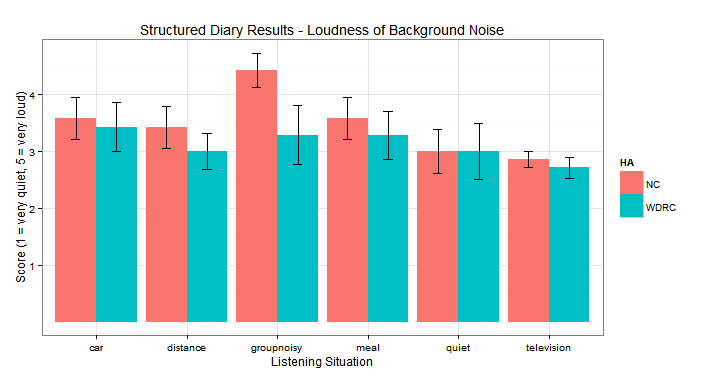
\includegraphics[height=3in]{chap5-structured-back-noise.png} \\
\caption[NCStudy2 structured diary results - loudness of background noise]{NCStudy2 structured diary results - loudness of background noise.  Error bars represent $\pm$ 1 SEM.  Participants tend to report that the loudness of background noise is too loud with the NC while speaking with a group of people in a noisy situation, while for the other situations there are no differences between the NC and WDRC.}
\label{chap5-struct-back-noise}
\end{center}
\end{figure}

\subsubsection{Feedback Form}
\paragraph{}Table 5.11 tabulates results from the feedback form.  On some questions, participants expressed no preference of one hearing aid over the other; in these cases, the observation was ignored when summing the amount of participants preferring WDRC or the NC.  Overall, 7 participants preferred WDRC, and 4 participants preferred the NC.  The main reasons for not liking the NC was that it was reported to be too loud relative to the WDRC, it produced uncomfortable sounds (most likely attributable to entrainment), and two participants complained that one side was louder than the other.  The main reasons for not liking the WDRC, was frequent feedback sounds, and a perceived lack of amplification.

%table
\begin{table}[htp]
\begin{center}
\begin{tabular}{lrrrrr}
  \hline
  Situation & NC Count & WDRC Count \\
  \hline
  Music        & 5 & 6 \\
  Speech in quiet & 4.5 & 6.5 \\
  Speech in noise & 3.5 & 7.5 \\
  Television & 5 & 6 \\
  Telephone & 3 & 8 \\
  Overall & 4 & 7 \\
   \hline
\end{tabular}
\end{center}
\caption{Hearing Aid Preference for Different Listening Situations}
\end{table}

\section{Discussion}
\paragraph{}The discussion of NCStudy2 proceeds in similar fashion to the discussion for NCStudy1.  First, potential limitations to the study design are outlined, followed by a discussion of results on the various tasks, so that the reader may interpret the results while keeping the study limitations in mind.

\subsection{Limitations}
\paragraph{}Unfortunately, despite being a much more controlled study than NCStudy1, there were still a few factors in the study that we were unable to control for, which may affect the interpretation of the results.

\subsubsection{Features}
\paragraph{}First, noise reduction and feedback cancellation had to be enabled on the test hearing aids, in order to ensure participants' acceptance of the hearing aids in their everyday listening environments.  Although the implementation of these features were, for the most part, identical between WDRC and NC, the constraint that these features must be identically implemented does not necessarily prevent them from contaminating the results.  The reason is that noise reduction and feedback cancellation could interact with the amplification algorithm, and for an ideal comparison of two amplification algorithms, all features on the hearing aids ought to be disabled.  During the design of the study, this issue was anticipated, and a solution was proposed to attempt to correct for this study design flaw.  The solution proposed the creation of 2 programs on participants' hearing aids (program 1: features enabled, and program 2: features disabled).  The intention was for program 1 to be the everyday listening program, and for program 2 to be used strictly in the testing environment.  The solution was sound, in theory, but after programming the hearing aids, it was determined that program 2 would be unusable, at least for the WDRC hearing aids, because there was an inordinate amount of feedback.  As a result, participants were told to use only program 1 on their hearing aids, and all participants complied.

In particular, the mistuned harmonic and timbre perception tasks were likely highly affected by the interaction between the amplification algorithm and the feedback canceller.  Some participants reported an additional ringing or an additional tone during the presentation of tonal stimuli while wearing the NC hearing aids (entrainment), and, as a result, found it difficult to perform to the best of their ability on these tasks.  By contrast, there were no entrainment-like symptoms reported for WDRC by any of the participants in the study.  The reason for entrainment occurring in the NC, but not the WDRC, could be due to the increased gain in the NC hearing aids, or slight differences in the implementation of the feedback canceller.  No statistically significant differences were observed between hearing aids on the mistuned harmonic and timbre perception tasks, but perhaps if entrainment was eliminated, or if features were entirely disabled and the proper care was taken to eliminate any source of feedback, this question could be addressed properly.  There was no effect of entrainment on the other tasks (the problem only occurs in response to sufficiently tonal inputs), so results from the other tasks may be interpreted knowing there was little or no effect of the feedback canceller on these tasks.

\subsubsection{Gain}
\paragraph{}Second, there appeared to be quite different amounts of gain between the NC and WDRC hearing aids, according to real ear measurements that were collected (Figures 5.3, 5.4, and 5.5).  In any comparison of hearing aid amplification algorithms, the gain is expected to differ between the algorithms, but perhaps not to the extent that the gain differed between hearing aids in the current study.  The WDRC hearing aids, though they were fit according to the DSL [i/o]* prescription, were given less gain than the prescribed target.  The WDRC software required the specialist to input the hearing aid experience of participants on a scale of 1 to 4 (1 = new hearing aid user, 4 = long time hearing aid user), and the specialist naturally selected a value of 1, and during the adjustment session was sometimes able to increase the value to 2.  Generally, in hearing aid fittings, it takes a while to adapt to the increased volume, so patients are often initially under-fit, and gain is gradually increased when patients ask for it, or when the specialist suggests it \cite{Brooks1973}.  By contrast, the NC gain is prescribed independent of any parameter specifying a user's hearing aid experience, which partly explains why more gain was given for the NC overall than the WDRC hearing aids.

\subsubsection{Adjustments}
\paragraph{}The software used to adjust the hearing aids also differs between hearing aid manufacturers, so when comparing two hearing aid technologies in the context of a study that has hearing aid adjustments, the efficacy of the adjustment depends on the clinician's familiarity with the software, and clinician's skill with one hearing aid technology versus the other.

\subsection{Conclusions from NCStudy2}
\subsubsection{Speech Intelligibility}
\paragraph{}A realistic speech in noise test did not show any significant differences in speech intelligibility between the two hearing aids, as well as a test of word recognition in quiet.  Vowel perception was also about the same between hearing aids.  However, the NC hearing aids performed poorer on consonant recognition.

Consonants that were especially worse with the NC were /d/, /h/ (mainly noise), /k/ (noise only), /r/ (mainly quiet), /s/, /t/, /w/ (noise only), and /z/ (mainly quiet).  These consonants fall into the categories of stop consonants (d, k, t), fricatives (h, s, z), and a couple of glides (r, w).  In order to better understand why consonant recognition was worse for these consonants, an overview of the acoustic features of these groups of consonants must first be presented.

The acoustic energy for stop consonants is relatively wideband, although /t/, and less so, /k/, have a lot of high frequency energy \cite{Hamill2008}.  Some other important characteristics of stop consonants are the stop gap, which is the length of time between the stop consonant and the next vowel, and the voice onset time, the time between the beginning of phoneme production and when the vocal folds start to vibrate.  The stop gap and voice onset times are useful for differentiating between voiced and unvoiced consonants.  Formant transition contours are also very important in the classification of stop consonants, in that stop consonants differ with respect to how a consonant's spectrum transitions into the subsequent vowel formants.  For instance, for the words /bet/, /det/, and /get/, /b/ has an ascending second formant transition, /d/ has a flat second formant transition, while /g/ has a descending second formant transition.

Fricatives are long in duration relative to the other consonants, and contain even more high frequency energy than stop consonants.  /s/ and /z/ contain the most high frequency energy out of all the English consonants.

Glides are very vowel-like, in that they mainly contain low frequency energy.  Glides also tend to be longer in duration, but /r/ is an exception to the rule.  Similar to the stop consonants, the formant transitions may be used as a cue for characterizing different glides.

Out of the consonants which the NC had trouble with, some common themes emerge.  One is that  the consonants mostly had high frequency energy, and formant transitions are especially important for these consonants to help with recognition. Therefore, it may be that the NC is not providing enough amplification at very high frequencies, or that the formant transitions are not being restored adequately.  Another possibility is that the prior or subsequent vowel is overamplified in the context of the VCV experiment, resulting in greater amounts of perceptual forward or backward masking of the consonant sound.

To investigate these hypotheses further, a sensible experiment would involve isolating each of these features in some stimulus, and experimentally manipulating these features one by one, in order to determine which of these features are distorting consonant perception for the NC hearing aid.

\subsubsection{Music Perception}
\paragraph{}One hearing aid did not result in superior frequency resolution, as measured by the mistuned harmonic task, nor was timbre perception more accurate with one hearing aid over another, unlike the trending result of favorable timbre perception for the NC in NCStudy1.  In NCStudy1, there were no complaints of entrainment during the procedure for either set of hearing aids, but in NCStudy2, there were complaints of entrainment, only for the NC hearing aids.  Thus, task performance could have been affected by entrainment for the NC, and for this reason it is difficult to interpret these results.

The most surprising result was that gap detection thresholds were consistently lower with WDRC than the NC hearing aids, indicating that temporal resolution is superior with WDRC.  There may be many reasons for this discrepancy in performance, but two reasons quickly come to mind.  One, is that compression is known to affect the detection of gaps in narrow bands of noise \cite{Glasberg1992, Moore2001}.  Specifically, when compression is applied to a narrow band noise stimulus, such as that used in the gap detection task employed in this thesis, one is able to detect smaller gaps in a noise band \cite{Glasberg1992}.  So, perhaps the difference in performance between the NC and WDRC on this task is due to less compression given by the NC, or a different type of compression used altogether (slow-acting, fast-acting).  The second possibility which could account for the worse performance for the NC hearing aids, is a difference in the amount of gain applied between the two hearing aid types.  Supposing that the NC gave more gain outside of the 1000 Hz region (where the noise band was centred), particularly just below the 1000 Hz region, then the noise band centred at 1000 Hz could be masked disproportionately more with the NC.

To evaluate the compression hypothesis, measures should be taken to quantify how much and what type of compression is being applied by the NC hearing aid.  To test the gain hypothesis, a gap detection experiment with noise bands centred at different frequencies could be designed, taking care to measure the amount of gain given to each participant in the experiment.

\subsubsection{Sound Localization}
\paragraph{}There was no significant main effect or interaction involving the hearing aid factor for the sound localization experiment.  However, looking at the localization error by stimulus type and angle graph (Figure 5.27), there did appear to be some differences between the NC and WDRC for high frequency stimuli presented close to centre (at 0$^\circ$, 15$^\circ$, and 30$^\circ$ angles), with the NC performing worse.  One potential reason for this discrepancy is that a couple of the NC hearing aid fittings gave asymmetrical gain between the two ears, perhaps distorting ILD cues for these participants, which are important for the localization of high frequencies.  To test this hypothesis, localization performance should be investigated on an individual basis.  One other possible reason is that the NC did not provide enough high frequency gain, reducing performance for the NC in the high frequency condition.  This hypothesis is supported by the fact that localization performance for the phone stimulus (which contains both high and low frequencies) also tended to be worse for the NC, yet localization performance for the low frequency stimulus was roughly equal.

\subsubsection{Subjective Measures}
\paragraph{}Several differences were observed between the two hearing aid types for the subjective measures collected in the current study.  The APHAB results indicated that background noise was overly loud with the NC compared to the WDRC, and certain sounds were especially loud (screeching tires, alarms/bells, running water, traffic noises, construction work, fire engines).  These findings were corroborated by evidence obtained from the structured diary used in the study.  The structured diary results indicated that background noise was too loud for the NC, but only when speaking with a group of people in a noisy situation.  One advantage that the NC had was that target speech tended to be closer to an optimal volume, as reported in the structured diary.  Overall sound quality and music quality was not reported to be better with one hearing aid type versus the other.

The results from the subjective measures suggest that the NC may not be providing enough compression, or that there is too much gain in the low frequencies and not enough in the high frequencies.  Background noise, which tends to have greater energy in the lower frequencies, might be overamplified with the NC.

\subsubsection{Overall}
\paragraph{}Taken together, the results from the whole study suggest that noise may be over-amplified and under-compressed with the NC.  A lack of compression, over-amplification of the low frequencies and potential under-amplification of the high frequencies are likely contributing to worse consonant perception, and worse temporal resolution for the NC hearing aid.   